\chapter{Como os animais se reproduzem}\label{ch:g4:animal-reproduction}

Em maio a lagoa fica barulhenta com o canto dos sapos; em junho ela
fica preta de \omterm{ex:g2:animals-grow-up:frog}{girinos}. O canto, ao que parece, era o começo da
história: a reprodução --- o jeito como os \omterm{def:g1:animals-around-us:animal}{animais} fazem a geração
seguinte --- segue regras que valem dos sapos aos elefantes, com
variações maravilhosas nos detalhes.

\section{São precisos dois}

\begin{definition}[Reprodução sexuada]\label{def:g4:animal-reproduction:sexual}
Nos \omterm{def:g1:animals-around-us:animal}{animais}, fazer filhotes quase sempre exige dois pais: uma
\emph{fêmea}\index{fêmea} e um \emph{macho}\index{macho}. A fêmea
produz \emph{células reprodutoras femininas}\index{célula
reprodutora feminina}; o macho produz
\emph{espermatozoides}\index{espermatozoide}. Um filhote começa
quando um espermatozoide se junta a uma célula reprodutora feminina
--- essa junção é a \emph{fecundação}\index{fecundação}. A
reprodução com dois pais se chama \emph{reprodução
sexuada}\index{reprodução sexuada}.
\end{definition}

\begin{example}[Por que os sapos cantam]\label{ex:g4:animal-reproduction:song}
O coro de maio são os \omterm{def:g4:animal-reproduction:sexual}{machos} chamando as \omterm{def:g4:animal-reproduction:sexual}{fêmeas} para a lagoa. Cada
casal solta então as células dele na água --- os óvulos da \omterm{def:g4:animal-reproduction:sexual}{fêmea}, os
\omterm{def:g4:animal-reproduction:sexual}{espermatozoides} do \omterm{def:g4:animal-reproduction:sexual}{macho} --- e ali acontece a \omterm{def:g4:animal-reproduction:sexual}{fecundação}. Os
pontinhos pretos na geleia poucos dias depois são os filhotes já
crescendo: o canto foi o passo um do ciclo do sapo do
\cref{ch:g2:animals-grow-up}.
\end{example}

\begin{omfigure}
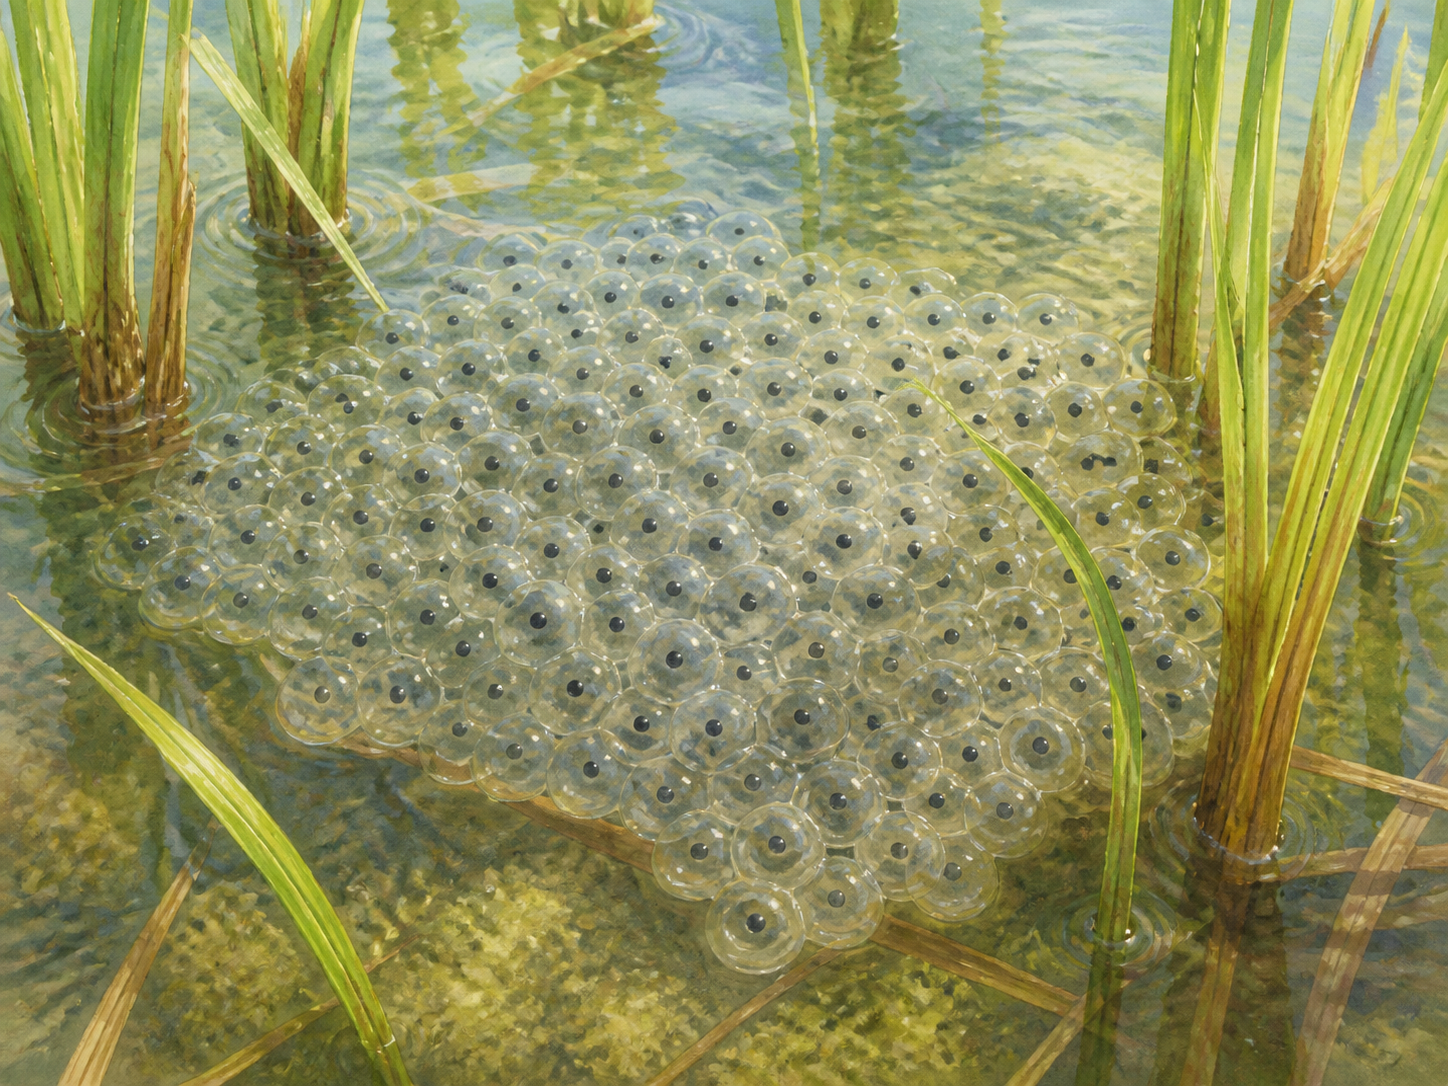
\includegraphics[width=0.56\linewidth]{images/book1/ai/g4-repro-frogspawn.png}

{\small Poucos dias depois do coro: a desova de sapo entre os
juncos, cada bola de geleia com um \omterm{def:g2:animals-grow-up:born}{ovo} fecundado e um sapinho
começando lá dentro.}
\end{omfigure}

\begin{remark}[Dois pais, sorte misturada]\label{rem:g4:animal-reproduction:mix}
Um filhote recebe alguma coisa de cada um dos pais --- e é por isso
que um potrinho pode ter a cor da mãe e a estrela branca do pai. O
que exatamente cada um dos pais entrega, e como, é uma das grandes
perguntas que ainda vêm neste livro; por enquanto, basta reparar que
todo \omterm{def:g1:animals-around-us:animal}{animal} nascido de \omterm{def:g4:animal-reproduction:sexual}{reprodução sexuada} tem dois pais e se parece
com os dois.
\end{remark}

\section{Ovos postos, ou filhotes de barriga}

\begin{definition}[Ovíparos e vivíparos]\label{def:g4:animal-reproduction:ovivivi}
Os dois jeitos de nascer da \cref{def:g2:animals-grow-up:born}
recebem agora os nomes científicos deles:
\begin{itemize}
  \item um \omterm{def:g1:animals-around-us:animal}{animal} é \emph{ovíparo}\index{ovíparo} se a \omterm{def:g4:animal-reproduction:sexual}{fêmea} põe
        \emph{\omterm{def:g2:animals-grow-up:born}{ovos}} e o filhote termina de crescer dentro do \omterm{def:g2:animals-grow-up:born}{ovo},
        fora do corpo dela: \omterm{prop:g3:sorting-living-things:groups}{aves}, quase todos os \omterm{prop:g3:sorting-living-things:groups}{peixes}, quase todos
        os \omterm{prop:g4:classifying-animals:classes}{répteis}, \omterm{prop:g3:sorting-living-things:groups}{anfíbios}, \omterm{prop:g3:sorting-living-things:groups}{insetos}, caracóis;
  \item um \omterm{def:g1:animals-around-us:animal}{animal} é \emph{vivíparo}\index{vivíparo} se o filhote
        cresce \emph{dentro do corpo da mãe}, alimentado por ela, e
        \emph{nasce de barriga}: quase todos os \omterm{prop:g3:sorting-living-things:groups}{mamíferos}.
\end{itemize}
\end{definition}

\begin{example}[Dois berçários]\label{ex:g4:animal-reproduction:nurseries}
O pintinho da galinha passa três semanas quentinhas num \omterm{def:g2:animals-grow-up:born}{ovo} com
casca, vivendo da gema (\cref{rem:g2:animals-grow-up:egg}); o
potrinho passa onze meses dentro da égua, alimentado sem parar pelo
corpo dela, e nasce pronto para ficar em pé em menos de uma hora. O
mesmo objetivo, dois berçários: um lanche embalado numa casca, e
serviço de quarto lá dentro.
\end{example}

\begin{proposition}[Onde acontece a fecundação]\label{prop:g4:animal-reproduction:where}
Para quem mora na água, como os \omterm{prop:g3:sorting-living-things:groups}{peixes} e os sapos, a \omterm{def:g4:animal-reproduction:sexual}{fecundação}
costuma acontecer \emph{na água}, fora do corpo da \omterm{def:g4:animal-reproduction:sexual}{fêmea} --- óvulos
e \omterm{def:g4:animal-reproduction:sexual}{espermatozoides} são soltos juntos e se encontram aos milhares.
Para os \omterm{def:g1:animals-around-us:animal}{animais} terrestres --- \omterm{prop:g3:sorting-living-things:groups}{aves}, \omterm{prop:g4:classifying-animals:classes}{répteis}, \omterm{prop:g3:sorting-living-things:groups}{mamíferos}, \omterm{prop:g3:sorting-living-things:groups}{insetos} ---
as células secariam ao ar livre, então o \omterm{def:g4:animal-reproduction:sexual}{macho} deposita os
\omterm{def:g4:animal-reproduction:sexual}{espermatozoides} \emph{dentro do corpo da \omterm{def:g4:animal-reproduction:sexual}{fêmea}} durante o
\emph{acasalamento}\index{acasalamento}, e a \omterm{def:g4:animal-reproduction:sexual}{fecundação} acontece ali.
\end{proposition}
\admitted

\section{Poucos filhotes e muito cuidado, ou muitos e nenhum}

\begin{proposition}[Duas estratégias para a geração seguinte]\label{prop:g4:animal-reproduction:strategies}
Compare os números: um bacalhau solta \emph{milhões} de \omterm{def:g2:animals-grow-up:born}{ovos} por ano
e não cuida de nenhum; uma elefanta tem \emph{um} filhote a cada
poucos anos e o protege por uma década. Entre esses extremos, uma
regra vale por todo o mundo \omterm{def:g1:animals-around-us:animal}{animal}: quanto mais filhotes uma espécie
produz, menos cuidado cada um recebe --- e quanto menos filhotes ela
produz, mais cada um é protegido e alimentado. As duas estratégias
dão certo: em média, sobrevivem filhotes suficientes para substituir
os pais.
\end{proposition}
\admitted

\begin{example}[Contando a lagoa]\label{ex:g4:animal-reproduction:pondcount}
A desova de um casal de sapos tem milhares de \omterm{def:g2:animals-grow-up:born}{ovos}. Garças,
peixinhos e larvas de libélula (veja o
\cref{ex:g3:food-chains:three}) comem \omterm{ex:g2:animals-grow-up:frog}{girinos} a primavera inteira
--- e, dos milhares, um punhado de sapinhos sobe a margem em julho.
A desova enorme não é desperdício: é a resposta do sapo aos perigos
da lagoa, sem nenhuma guarda dos pais.
\end{example}

\begin{example}[O outro extremo]\label{ex:g4:animal-reproduction:whalecalf}
O filhote de baleia nasce sozinho, nada logo ao lado da mãe, bebe o
\omterm{def:g2:animals-grow-up:born}{leite} gordo dela durante muitos meses e é defendido de todo perigo.
Um filhote de cada vez --- mas esse um recebe tudo. Os \omterm{prop:g3:sorting-living-things:groups}{mamíferos},
com o \omterm{def:g2:animals-grow-up:born}{leite} deles (\cref{def:g2:animals-grow-up:born}), são os
grandes especialistas da estratégia de poucos e bem cuidados.
\end{example}

\begin{method}[Ler a estratégia de uma espécie]\label{met:g4:animal-reproduction:read}
Diante de uma espécie, pergunte:
\begin{enumerate}
  \item Quantos filhotes de cada vez --- um, uma dúzia, milhares?
  \item Quem protege e alimenta esses filhotes --- os dois pais, a
        mãe, ninguém?
  \item Onde eles começam --- num \omterm{def:g2:animals-grow-up:born}{ovo} fora, ou crescendo dentro?
  \item Confira o equilíbrio da
        \cref{prop:g4:animal-reproduction:strategies}: muitos
        filhotes com pouco cuidado, ou poucos com muito.
\end{enumerate}
\end{method}

\section{Exercícios}

\begin{exercise}[$\star$]\label{exo:g4:animal-reproduction:1}
O que é a \omterm{def:g4:animal-reproduction:sexual}{fecundação}? Que célula vem de cada um dos pais?
\end{exercise}

\begin{exercise}[$\star$]\label{exo:g4:animal-reproduction:2}
Defina \omterm{def:g4:animal-reproduction:ovivivi}{ovíparo} e \omterm{def:g4:animal-reproduction:ovivivi}{vivíparo}, com dois \omterm{def:g1:animals-around-us:animal}{animais} de cada tipo.
\end{exercise}

\begin{exercise}[$\star$]\label{exo:g4:animal-reproduction:3}
Por que os sapos estavam cantando em maio? Reconte a história da
lagoa em três passos.
\end{exercise}

\begin{exercise}[$\star$]\label{exo:g4:animal-reproduction:4}
Onde acontece a \omterm{def:g4:animal-reproduction:sexual}{fecundação} para a truta, e onde para a galinha? Por
que essa diferença, segundo a
\cref{prop:g4:animal-reproduction:where}?
\end{exercise}

\begin{exercise}[$\star$]\label{exo:g4:animal-reproduction:5}
Compare os berçários do pintinho e do potrinho: onde cada um cresce
e o que o alimenta?
\end{exercise}

\begin{exercise}[$\star$]\label{exo:g4:animal-reproduction:6}
Enuncie a regra que liga o número de filhotes ao cuidado que eles
recebem. Dê os dois exemplos extremos do capítulo.
\end{exercise}

\begin{exercise}[$\star$]\label{exo:g4:animal-reproduction:7}
Os milhões de \omterm{def:g2:animals-grow-up:born}{ovos} do bacalhau quase nunca viram bacalhaus adultos.
Por que mesmo assim a estratégia dá certo?
\end{exercise}

\begin{exercise}[$\star$]\label{exo:g4:animal-reproduction:8}
Rode o \cref{met:g4:animal-reproduction:read} na gata: ninhada
típica de uns cinco filhotes, amamentados e protegidos pela mãe
durante semanas, crescidos dentro dela. De que lado da estratégia
ela está mais perto?
\end{exercise}

\begin{exercise}[$\star\star$]\label{exo:g4:animal-reproduction:9}
Um potrinho muitas vezes se parece com os dois pais ao mesmo tempo.
O que isso mostra sobre o que o filhote recebe, segundo a
\cref{rem:g4:animal-reproduction:mix}?
\end{exercise}

\begin{exercise}[$\star\star$]\label{exo:g4:animal-reproduction:10}
O \omterm{def:g4:animal-reproduction:sexual}{macho} do peixinho-espinho constrói um ninho, abana os \omterm{def:g2:animals-grow-up:born}{ovos} e
espanta os invasores --- uma dedicação rara para um peixe. Usando a
\cref{prop:g4:animal-reproduction:strategies}, o que você preveria
sobre o tamanho da desova dele, comparada com os milhões do
bacalhau?
\end{exercise}

\begin{exercise}[$\star\star\star$]\label{exo:g4:animal-reproduction:11}
As tartarugas marinhas rastejam até a praia para enterrar os \omterm{def:g2:animals-grow-up:born}{ovos} na
areia quente e depois voltam para o mar. Ovíparas ou vivíparas? Com
cuidado ou sem? E por que esse réptil, nadador a vida inteira,
precisa mesmo assim pôr os \omterm{def:g2:animals-grow-up:born}{ovos} em \emph{terra}? (Use as
características dos \omterm{prop:g4:classifying-animals:classes}{répteis} da
\cref{prop:g4:classifying-animals:classes}.)
\end{exercise}
